\usepackage{amsmath,interval,amssymb,xcolor,manfnt,tikz}

\makeatletter
\renewcommand\subsection{\@startsection{subsection}{3}{\z@}%
                                     {-3.25ex\@plus -1ex \@minus -.2ex}%
                                     {-1.5ex \@plus .2ex}%
                                     {\normalfont\normalsize\bfseries}}
\makeatother
\addtolength{\parskip}{.5\baselineskip}
\renewcommand*{\thefootnote}{\fnsymbol{footnote}}

\DeclareMathOperator{\Dirac}{Dirac}
\DeclareMathOperator{\expit}{expit}
\DeclareMathOperator{\logit}{logit}
\DeclareMathOperator{\Rem}{Rem}
\DeclareMathOperator{\Var}{Var}

\newsavebox\gearbox
\newcommand{\gearmacro}[5]{%
  % #1 number of teeths
  % #2 radius intern
  % #3 radius extern
  % #4 angle from start to end of the first arc
  % #5 angle to decale the second arc from the first 
  \foreach \i in {1,...,#1} {%
    [rotate=(\i-1)*360/#1]  (0:#2)  arc (0:#4:#2) {[rounded corners=1.5pt]
      -- (#4+#5:#3)  arc (#4+#5:360/#1-#5:#3)} --  (360/#1:#2)
  }}  
\newcommand{\makegear}{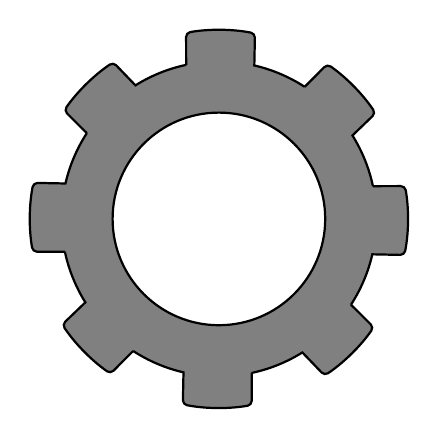
\begin{tikzpicture}
    \fill[gray] (0,0) circle (2cm);
    \draw[thick,rotate=12,fill=gray] \gearmacro{8}{2}{2.4}{20}{2};
    \draw[thick,fill=white] (0cm,0cm) circle(1.35cm);
  \end{tikzpicture}}
\sbox\gearbox{\resizebox{!}{2em}{\makegear}}
\newcommand{\gear}{\usebox{\gearbox}\;}

\newcommand{\bbO}{\mathbb{O}}
\newcommand{\bbP}{\mathbb{P}}
\newcommand{\bbR}{\mathbb{R}}
\newcommand{\calF}{\mathcal{F}}
\newcommand{\calM}{\mathcal{M}}
\newcommand{\calO}{\mathcal{O}}
\newcommand{\Exp}{\textrm{E}}
\newcommand{\Gbar}{\bar{G}}
\newcommand{\one}{\textbf{1}}
\renewcommand{\Pr}{\textrm{Pr}}
\newcommand{\Psihat}{\widehat{\Psi}}
\newcommand{\Qbar}{\bar{Q}}
\newcommand{\tcg}[1]{\textcolor{olive}{#1}}

\allowdisplaybreaks

%%% Local Variables:
%%% mode: latex
%%% TeX-master: t
%%% End:
